\section{Learning function-valued functions}
In this section we show how to used \acs{OVK} in hand with the \acs{ORFF}
framework to learn function valued function. We focus on two application cases:
quantile regression and one-class classification. This section is rather an
informal (but detailed) discussion on ideas that we hope will lead to new
publications.
\subsection{Quantile regression}
\label{subsec:quantile_regression}
This introduction to quantile regression is adapted from the paper
\citet{sangnier2016joint}, As we have seen in the introductory
\cref{ch:motivations}, a standard task in machine learning is to estimate the
conditional expectation $f(x)=\expectation_{\probability}[Y | X = x]$, where
$(X,Y)\sim\probability$ with some function belonging to a hypothesis space
$f\in\mathcal{F}$. Yet, many sensitive applications need more than the expected
valued of the relationship between random variables. To control the
\say{quality} of the predicted value from an input $x$, fields such as
economics, medicine, physics or social science require to have acces to the
different quantile to model the distribution around the mean
$f(x)\in\mathbb{R}$ and strengthen their analysis.
\paragraph{}
Here we are interested in learning and predicting simultaneously \emph{all} the
quantiles on the compact $[0, 1]$, of the scalar-valued random variable $Y|X$.
We place ourselve in the setting of conditional quantile regression by
minimization of the pinball loss \citep{koenker1978regression}. For $\tau\in[0,
1]$ the pinball loss reads
\begin{dmath*}
    L_{\tau}(x, f, y) = \max(\tau \left(f(x) - y\right), (\tau - 1) \left(f(x)
    - y\right)).
\end{dmath*}
In a nutshell, this loss has been introduced by noticing that finding the
optimal location parameter $\mu = f(x)$ in the $\ell_1$ loss $L(x, f,
y)=\abs{f(x) - y}$ yields an estimator of the unconditional median
\citep{koenker1978regression}. Recently \citet{sangnier2016joint} proposed to
learn simultaneously many quantiles by minimizing the multiquantile loss
function. Given a vector of quantiles $\boldsymbol{\tau} = (\tau_1, \dots
\tau_p)\in\mathbb{R}^p$
\begin{dmath*}
    L_{\boldsymbol{\tau}}(x, f, y) = \sum_{i=1}^p \max(\boldsymbol{\tau}_i
    \left(f(x)_i - y\right), (\boldsymbol{\tau}_i - 1)\left(f(x)_i - y\right)).
\end{dmath*}
We see that now it is necessary for $f(x)\in\mathbb{R}^p$ to be vector-valued.
In this work we push further the idea by considering that $f(x)$ is a function
of an arbitrary quantile $\tau\in[0, 1]$. Thus we view $f$ as a vector valued
function $f:\mathbb{R} \to ([0, 1] \to \mathbb{R})$. For the sake of simplicity
we note $f(x)=f_x$ and introduce the generalized the pinball loss
\begin{dmath}
    \label{eq:loss_pinball}
    L(x, f, y) = \int_{[0, 1]} \max(\tau \left(f_x(\tau) - y\right), (\tau -
    1)\left(f_x(\tau) - y)\right) d\tau.
\end{dmath}

\subsection{Functional output data}
Pioneer work on learning function valued function has been done by
\citet{kadri2015operator}. Inspired by them we developp an \acs{ORFF}
methodology to learn functional data where the outputs are functions that we
suppose living in a \acs{RKHS}.
\paragraph{}
Namely, we suppose that the image of a funtion $f$ $f(x) \in
\mathcal{H}_{k_{\mathcal{T}}}$ has value in a \acs{RKHS}, where
$k_{\mathcal{T}}:\mathcal{T}^2\to\mathbb{R}$ is a scalar-valued kernel and
$\mathcal{H}_{k_{\mathcal{T}}}$ is corresponding \acs{RKHS}. From this
hypothesis we see that
\begin{dmath*}
    f_x(\tau) = \inner{f(x), k_{\mathcal{T}}(\cdot,
    \tau)}_{\mathcal{H}_{k_{\mathcal{T}}}}
\end{dmath*}
If we add the second hypothesis that $f\in\mathcal{H}_K$, where $\mathcal{H}_K$
is a \emph{\acl{vv-RKHS}} for some \acl{OVK} $K$. \Citet{Carmeli2010} showed in
example $6$ page $17$-$18$ that in this case the operator $K$ is given by
\begin{dmath}
    \label{eq:functional_kernel}
    K =
    \begin{cases}
        \mathcal{X} \times \mathcal{X} & \to
        \mathcal{L}(\mathcal{H}_{k_{\mathcal{T}}}) \\
        x, z & \mapsto k_{\mathcal{X}}(x, z) I_{\mathcal{H}_{k_{\mathcal{T}}}},
    \end{cases}
\end{dmath}
where $k:\mathcal{X}\times\mathcal{X} \to \mathbb{R}$ is another scalar-valued
kernel. Moreover \citet{Carmeli2010} showed in example $7$ page $18$-$19$ that
the \acs{vv-RKHS} induced by $K$ is the same \acs{RKHS} than the one induced by
the kernel $K'$ defined as follow for some measure $\mu$ with support
$\mathcal{T}$.
\begin{dmath*}
    K' =
    \begin{cases}
        \mathcal{X} \times \mathcal{X} & \to
        \mathcal{L}\left(L^2(\mathcal{T}, \mu)\right) \\
        x, z & \mapsto k_{\mathcal{X}}(x, z)
        \int_{\mathcal{T}}k_{\mathcal{T}}(\cdot, \tau)g(\tau)d\mu(\tau).
    \end{cases}
\end{dmath*}
This is exactly the decomposable kernel introduced in
\cref{def:hilbert_schmidt_integral_kernel} in \cref{ch:motivations}. Because
The \acsp{RKHS} induced by $K$ and $K'$ are the same, we can either view its
elements as functions from $\mathcal{X}$ into $\mathcal{H}_{k_{\mathcal{T}}}$
(through $\mathcal{H}_K$) or as function from $\mathcal{X}$ into
$L^2(\mathcal{T}, \mu)$ (through $\mathcal{H}_{K'}$).

\subsection{ORFF for functional output data}
Because $\mathcal{Y}=\mathcal{H}_{k_{\mathcal{T}}}$ is a proper (infinite
dimensional) Hilbert space, we can apply the \acs{ORFF} methodology. Let
$k_{\mathcal{X}}$ be a scalar Mercer kernel and $\mathcal{X}=\mathbb{R}$. Then
by \cref{cr:ORFF-map-kernel} applied to the decomposable kernel (see
\cref{subsec:examples_ORFF}) we have the following approximate feature map for
$K$ defined in \cref{eq:functional_kernel}:
\begin{dmath*}
    \tildePhi{\omega}(x)y = \frac{1}{\sqrt{D}}\Vect_{j=1}^D
    \begin{pmatrix}
        \cos(x \omega_j) B^\adjoint y \\
        \sin(x \omega_j) B^\adjoint y
    \end{pmatrix} \condition{$\omega_j \sim \FT{k_{\mathcal{X}}}$
    \ac{iid}}
\end{dmath*}
where $BB^\adjoint = I_{\mathcal{H}_{k_{\mathcal{T}}}}$ and
$y\in\mathcal{H}_{k_{\mathcal{T}}}$. At this point we could choose
$B=I_{\mathcal{H}_{k_{\mathcal{T}}}}$. However this is not really useful since
it would make the redescription space $\widetilde{\mathcal{H}}=\Vect_{j=1}^D
\mathcal{H}_{k_{\mathcal{T}}}$, which is a direct sum of infinite dimensional
\acs{RKHS}. Yet since $\mathcal{H}_{k_{\mathcal{T}}}$ is a \acs{RKHS},
according to \cref{pr:feature_operator} it is possible to define a feature
operator $W:\mathcal{H}\to\mathcal{H}_{k_{\mathcal{T}}}$ such that
$(Wg)(\tau)=\Phi_\tau^\adjoint g$. 
\maxdeadcycles=10000
\afterpage{%
\begin{landscape}
    \begin{figure}[htp]
        \centering
        \resizebox{.8\textheight}{!}{%
        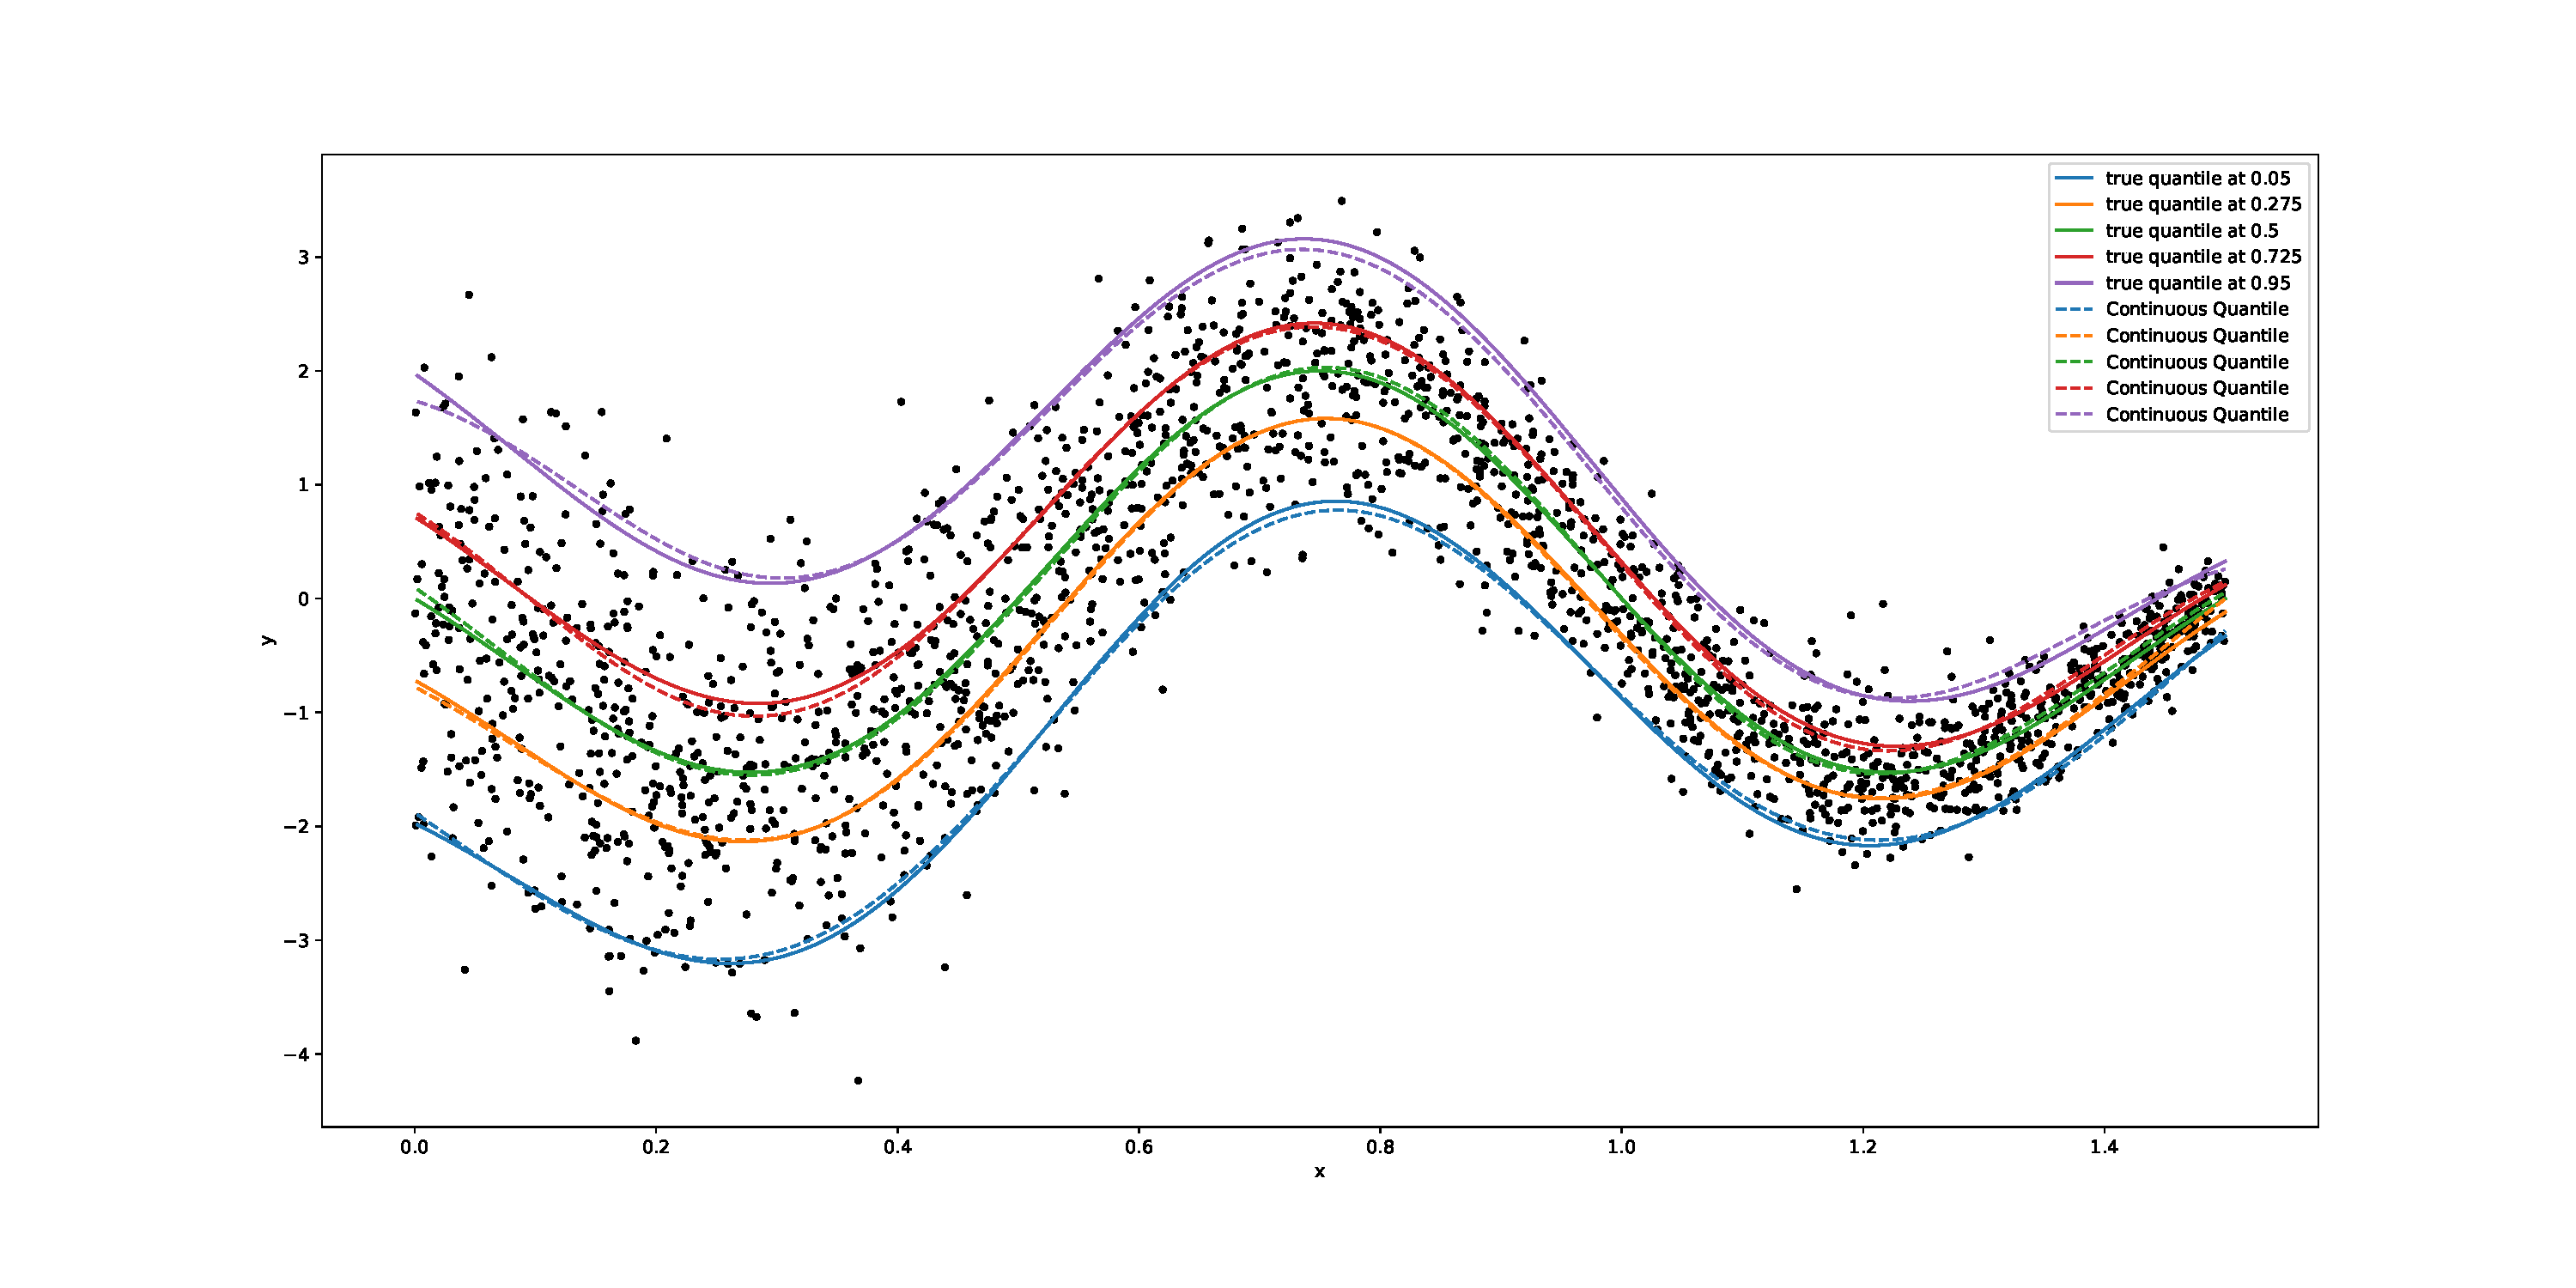
\includegraphics{./gfx/quantile_orff.pdf}}
        \caption{Learning a continuous quantile function with ORFF
        regression. \label{fig:quantile_orff}}
    \end{figure}
    \clearpage
    \begin{figure}[htp]
        \centering\resizebox{.8\textheight}{!}{%
        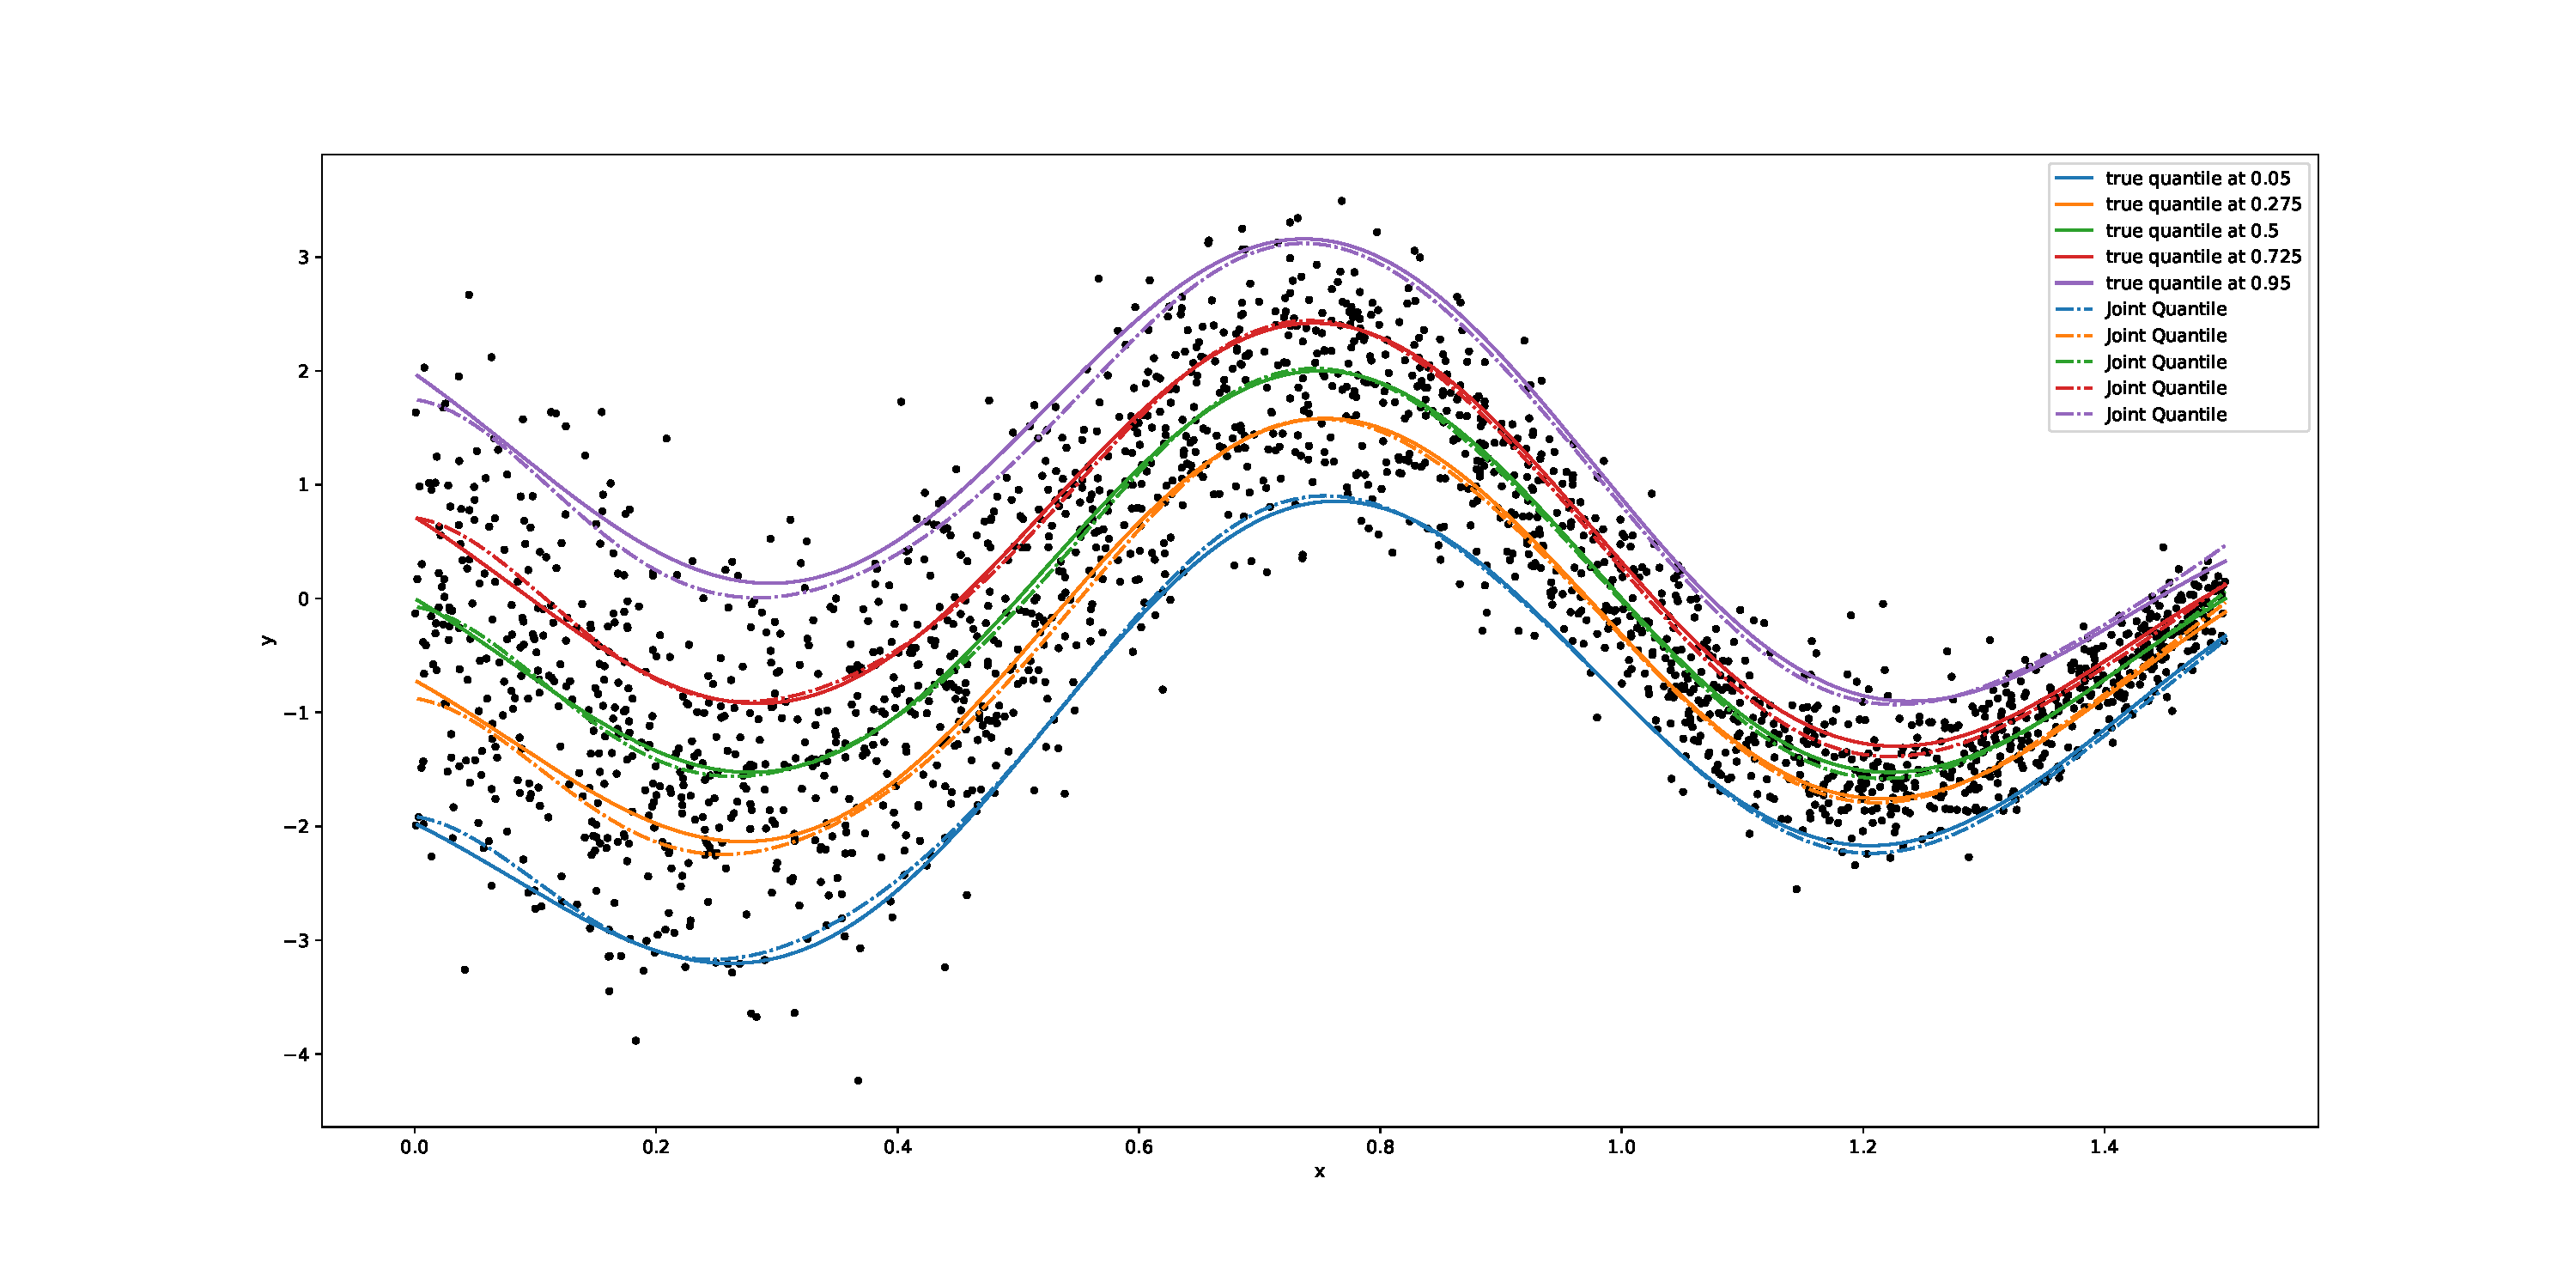
\includegraphics{./gfx/quantile_joint.pdf}}
        \caption{Learning many quantile with joint OVK regression.
        \label{fig:quantile_joint}}
    \end{figure}
\end{landscape}}
Moreover $W^\adjoint W$ is the identity on
$\Ima \Phi_{\tau}$ which is here $\mathcal{H}_{k_{\mathcal{T}}}$. (see the
proof of \cref{pr:feature_operator} and \citet{Carmeli2010}). Thus we can
choose $\Phi_\tau=\Phi(\tau)$ to be the functional Fourier feature map
associated to $k_{\mathcal{T}}$ defined in \cref{pr:fourier_feature_map}.  Then
we have $BB^\adjoint = I_{\mathcal{H}_{k_{\mathcal{T}}}} = W^\adjoint W$.  Thus
we can choose $B^\adjoint = W = \Phi(\cdot)^\adjoint$ and the approximate
feature map reads 
\begin{dmath*}
    \tildePhi{\omega}(x)\in \mathcal{L}\left(\mathcal{H}_{k_{\mathcal{T}}};
    \Vect_{j=1}^D L^2\left(\dual{\mathcal{T}},
    \probability_{\dual{\Haar},\rho}\right)\right)
\end{dmath*}
and
\begin{dmath*}
    (\tildePhi{\omega}(x)g)(\tau) = \frac{1}{\sqrt{D}}\Vect_{j=1}^D
    \begin{pmatrix}
        \cos(x \omega_j) \Phi(\tau)^\adjoint g \\
        \sin(x \omega_j) \Phi(\tau)^\adjoint g
    \end{pmatrix} \condition{$\omega_j \sim \FT{k_{\mathcal{X}}}$
    \ac{iid}}
\end{dmath*}
Then as proposed in \cref{ch:operator-valued_random_fourier_features} we can
Monte-Carlo sample the functional feature map $\Phi(\tau)$ and obtain the 
\acs{ORFF} map 
\begin{dmath*}
    \left(\widetilde{\tildePhi{\omega}}(x)g\right)(\tau) =
    \frac{1}{\sqrt{DD'}}\Vect_{j=1}^D
    \begin{pmatrix}
        \cos(x \omega_j) \sum_{k=1}^{D'}
        \left(\cos(\tau \omega_k') + \sin(\tau \omega_k')\right)g(\omega_k') \\
        \sin(x \omega_j) \sum_{k=1}^{D'}
        \left(\cos(\tau \omega_k') + \sin(\tau \omega_k')\right)g(\omega_k')
    \end{pmatrix} \condition{$\omega_j \sim \FT{k_{\mathcal{X}}}$
    \acs{iid} and $\omega_k'\sim \FT{k_{\mathcal{T}}}$ \acs{iid}.}
\end{dmath*}
where $g\in L^2\left(\dual{\mathcal{T}}, \probability_{\dual{\Haar},
\rho}\right)$ and $\tau\in\mathbb{R}$. If we note 
\begin{dmath*}
    G = 
    \begin{pmatrix}
        g(\omega_1') & \dots & g(\omega_{D'}') 
    \end{pmatrix}^\adjoint \hiderel{\in} \mathbb{R}^{D'}
\end{dmath*}
we can define
\begin{dmath*}
    \left(\widetilde{\tildePhi{\omega}}(x)G\right)(\tau) =
    \frac{1}{\sqrt{DD'}}\Vect_{j=1}^D
    \begin{pmatrix}
        \cos(x \omega_j) \sum_{k=1}^{D'}
        \left(\cos(\tau \omega_k') + \sin(\tau \omega_k')\right)G_k \\
        \sin(x \omega_j) \sum_{k=1}^{D'}
        \left(\cos(\tau \omega_k') + \sin(\tau \omega_k')\right)G_k
    \end{pmatrix} \condition{$\omega_j \sim \FT{k_{\mathcal{X}}}$
    \acs{iid} and $\omega_k'\sim \FT{k_{\mathcal{T}}}$ \acs{iid}.}
\end{dmath*}
Then it is easy to verify that the adjoint operator is given by
\begin{dmath*}
    \left(\widetilde{\tildePhi{\omega}}(x)^\adjoint \theta\right)(\tau) =
    \frac{1}{\sqrt{DD'}} \sum_{j=1}^D \left(\cos(x\omega_j) +
    \sin(x\omega_j)\right) \left(\Vect_{k=1}^{D'}
    \begin{pmatrix}
        \cos(\tau \omega_k') \\
        \sin(\tau \omega_k')
    \end{pmatrix}\right)^\adjoint \theta_j
    = \frac{1}{\sqrt{DD'}} \sum_{j=1}^D \left(\cos(x\omega_j) +
    \sin(x\omega_j)\right) \theta_{jk} \left( \cos(\tau \omega_k') + \sin(\tau
    \omega_k')\right)
    \condition{$\omega_j \sim \FT{k_{\mathcal{X}}}$
    \acs{iid} and $\omega_k'\sim \FT{k_{\mathcal{T}}}$ \acs{iid}.}
\end{dmath*}
where $\theta_k\in\mathbb{R}^{D'}$, for all $k \in \mathbb{N}^*_D$ and
$\theta_{jk}\in\mathbb{R}$ for all $j \in \mathbb{N}^*_D$ and all $k \in
\mathbb{N}^*_{D'}$. The above equations can be rewritten in matrix form which
results in the following conjecture.
\begin{conjecture}
    \label{cj:functional_orff}
    If $\tildephi{\omega}_{\mathcal{X}}$ is an \acs{RFF} for
    $\widetilde{k}_{\mathcal{X}}$ such that
    $\tildephi{\omega}(x)\in\mathbb{R}^D$ and $\tildephi{\omega}_{\mathcal{T}}$
    is an \acs{RFF} for $\widetilde{k}_{\mathcal{T}}$, such that
    $\tildephi{\omega}(\tau)\in\mathbb{R}^{D'}$ then an \acs{ORFF} map for
    \begin{dmath*}
        K(x, z) = k_{\mathcal{X}}(x, z) I_{\mathcal{H}_{k_{\mathcal{T}}}}
    \end{dmath*}
    is given for all $x\in\mathbb{R}$, all $\tau\in\mathbb{R}$ and all
    $\Theta\in\mathcal{M}_{D,D'}(\mathbb{R})$ by
    \begin{dmath*}
        \left(\tildePhi{\omega}_K(x)^\adjoint \Theta \right)(\tau) =
        \tildephi{\omega}_{\mathcal{X}}(x)^\adjoint \Theta
        \tildephi{\omega}_{\mathcal{T}}(\tau)
    \end{dmath*}
    and
    \begin{dmath*}
        \left(\tildePhi{\omega}_K(x) G\right)(\tau) =
        \tildephi{\omega}_{\mathcal{X}}(x)
        \tildephi{\omega}_{\mathcal{T}}(\tau)^\adjoint G,
    \end{dmath*}
    where $g\in\mathbb{R}^{D'}$.
    %but more intestingly, given $y\in\mathbb{R}$,
    %\begin{dmath*}
        %\tildePhi{\omega}_K(x, \tau)^\adjoint y =
        %y \tildephi{\omega}_{\mathcal{X}}(x)
        %\tildephi{\omega}_{\mathcal{T}}(\tau)^\adjoint.
    %\end{dmath*}
\end{conjecture}
Moreover if one defines $\tildePhi{\omega}_K(x,
\tau) = \left(\tildePhi{\omega}_K(x)^\adjoint \Theta \right)(\tau)$ one
have of course
\begin{dmath*}
    \tildePhi{\omega}_K(x, \tau)^\adjoint \Theta =
    \tildephi{\omega}_{\mathcal{X}}(x)^\adjoint \Theta
    \tildephi{\omega}_{\mathcal{T}}(\tau)
\end{dmath*}
\subsection{Many quantile regression}
From the loss defined in \cref{eq:loss_pinball} we defined the regularized risk
using the \say{continuous} pinball loss for the quantile regression problem.
For all $f\in\mathcal{H}_K$,
\begin{dmath*}
    J_{\lambda}(f) =
    \frac{1}{N}\sum_{i=1}^N\int_{[0,1]}\left(
    \begin{cases}
        \tau\left(f_{x_i}(\tau) - y_i\right) & \text{if } f_{x_i}(\tau) \ge y_i
        \\
        (1 - \tau)\left(y_i - f_{x_i}(\tau)\right) & \text{otherwise} 
    \end{cases} \right)+ \lambda
    \norm{f}_K^2.
\end{dmath*}
The issue with the above risk is that the different quantile for a given point
$x\in\mathbb{R}$ may cross \citet{sangnier2016joint}. To avoid this to happen
we need to force the function $f_x(\tau)$ to be \emph{increasing} in $\tau$ for
any $x\in\mathbb{R}$.  Because a decreasing function has a negative derivative
we can add a penalty term to the risk to avoid $f_x(\tau)$ to be decreasing in
$\tau$.
\begin{dmath*}
    \Omega_{cross}(f) = - \min\left(\frac{\partial
    f_{x_i}}{\partial\tau}(\tau),
    0\right)
\end{dmath*}
Thus the regularized risk with the no crossing constraint is
\begin{dmath*}
    J_{\lambda_1, \lambda_2}(f) =
    \frac{1}{N}\sum_{i=1}^N\int_{[0,1]}\left(
    \begin{cases} 
        \tau \left(f_{x_i}(\tau) - y_i\right) & \text{if } f_{x_i}(\tau) \ge
        y_i \\
        (1 - \tau)\left(y_i - f_{x_i}(\tau)\right) & \text{otherwise}
    \end{cases} -
    \lambda_1 \min\left(\frac{\partial f_{x_i}}{\partial\tau}(\tau), 0\right)
    \right)+ \lambda_2 \norm{f}_K^2.
\end{dmath*}
Eventually we replace the integral by a Monte-Carlo sampling with the uniform
law $\mathcal{U}([0, 1])$ and plug in the approximate function of $f$ using the
\acs{ORFF} map proposed in \cref{cj:functional_orff}. The final optimzation
problem reads
\begin{dmath*}
    J_{\lambda_1, \lambda_2}(\Theta) =
    \frac{1}{NT}\sum_{i=1}^N\sum_{t=1}^T\left(
    \begin{cases} \tau_t
        \left(\widetilde{f}_{x_i}(\tau_t) - y_i\right) & \text{if }
        \widetilde{f}_{x_i}(\tau_t) \ge y_i \\
        (1 - \tau_t)\left(y_i - f_{x_i}(\tau_t)\right) & \text{otherwise} 
    \end{cases} - \lambda_1
    \min\left(\frac{\partial \widetilde{f}_{x_i}}{\partial\tau}(\tau_t),
    0\right) \right)+ \lambda_2 \norm{\Theta}_{fro}^2.
\end{dmath*}
where $\widetilde{f}_{x}(\tau)=\tildephi{\omega}_{\mathcal{X}}(x)^\adjoint
\Theta \tildephi{\omega}_{\mathcal{T}}(\tau)$, $\tau_t \sim \mathcal{U}([0,
1])$ and
\begin{dmath*}
    \frac{\partial \widetilde{f}_{x}}{\partial\tau}(\tau)
    = \tildephi{\omega}_{\mathcal{X}}(x)^\adjoint \Theta \frac{\partial
    \tildephi{\omega}_{\mathcal{T}}}{\partial \tau}(\tau)
    = \tildephi{\omega}_{\mathcal{X}}(x)^\adjoint \Theta \Vect_{k=1}^{D'}
    \begin{pmatrix}
        -\omega_k' \sin(\omega_k' x) \\
         \omega_k' \cos(\omega_k' x)
    \end{pmatrix} \condition{$\omega_k' \sim \FT{k_{\mathcal{T}}}$ \acs{iid}.}
\end{dmath*}
\subsubsection{Some results}
We minimize the quantity $J_{\lambda_1, \lambda_2}(\Theta)$ on a toy dataset: a
since wave with some heteroscedastic noise. First we compare our methodology to
the joint quantile regression proposed in \citet{sangnier2016joint}. We
generate $N=2500$ for the train set and $N'=1000$ points for the test set and
use a gaussian kernel for both $k_{\mathcal{X}}$ and $k_{\mathcal{T}}$. We
choosed $\sigma_{\mathcal{X}} = 0.25$ and $\sigma_{\mathcal{T}}$ is set to be
the median of the pairwise distance of the $\tau_t$'s drawn randomly from
$\mathcal{U}([0, 1])$. Notice that $J_{\lambda_1, \lambda_2}(\Theta)$ is convex
in $\Theta$. To avoid computing complex gradients and by lack of time, we used
Tensorflow \citep{abadi2016tensorflow} to perform a gradient descent (with
RMSProp \citep{tieleman2012lecture}) with automatic symbolic differentiation.
\Cref{fig:quantile_orff} show the result for the quantile at $0.05$, $0.275$,
$0.5$, $0.775$ and $0.95$ using the \acs{ORFF} methodology. 
\afterpage{%
\begin{landscape}
    \begin{figure}[htp]
        \centering
        \resizebox{.8\textheight}{!}{%
        \includegraphics{./gfx/quantile_continuous.pgf}}
        \caption{Learning a continuous quantile function with ORFF
        regression. \label{fig:quantile_continuous}}
    \end{figure}
\end{landscape}}
\Cref{fig:quantile_joint} shows the joint quantile regression of
\citet{sangnier2016joint} on the same dataset. Not only our method matches the
the performaces of \citet{sangnier2016joint}\footnote{We reported an error
computed with the pinball loss on the test set of $0.818$ for our method and
$0.817$ for joint regression (note that we don't report here an average on many
experiments to avoid randomness introduced by the random features, but the
results seems robut in practice.)} but we cut down the computation time from
circa $1330$ seconds to circa $30$ seconds (training and testing).  Moreover on
contrary to \citet{sangnier2016joint} we have access to all the quantile of the
model (see \cref{fig:quantile_continuous}).

\subsection{One class SVM revisited}
We also propose an extension of the celebrated \acf{OCSVM} so that it
possible to learn jointly all the level sets.  One-class classification, also
known as unary classification, tries to identify objects of a specific class
amongst all objects, by learning from a training set containing only the
objects of that class.  In this framework, we assume that we only observe
examples of one class (referred to as the inlier class).  The second class is
called outlier class.  We turn our attention to the \acs{OCSVM}
\citet{Scholkopf2001} which extends the \ac{SVM} methodology
\citep{Cortes1995,Shawe2004} to handle training using only inliers. 
\paragraph{}
We recall that given an hyperparameter $\nu\in [0,1]$ that controls the
proportion of inlier, given as scalar kernel $k$, the \acs{OCSVM} problem reads
\begin{dmath*}
    \argmin_{f\in\mathcal{H}_k, \rho \in \mathbb{R}} \frac{1}{2}
    \norm{f}_{\mathcal{H}_k}^2 - \nu \rho + \frac{1}{N} \sum_{i=1}^N \max(\rho
    - f(x_i), 0)
\end{dmath*}
As in \cref{subsec:quantile_regression} we can rewrite the optimization problem
as an integral over all the value of $\nu$ and suppose that $f$ is
function-valued (a function of $\nu$). Moreover $\tau$ must also change its
value according to $\mu$. Thus given a kernel $k_{\mathcal{X}}$ on the inputs
$x\in\mathbb{R}^d$ with its approximate feature map
$\tildephi{\omega}_{\mathcal{X}}$ and a kernel $k_{\mathcal{T}}$ on the level
sets with its approximate feature map $\tildephi{\omega}_{\mathcal{T}}$, we
define the continuous one-class SVM problem as
\begin{dmath*}
    \argmin_{f
    \in\mathcal{H}_K,\tau\in\mathcal{H}_{k_{\mathcal{\tau}}}}\frac{1}{N}
    \sum_{i=1}^N\int_{[0,1]}\max\left(0, \tau(\nu) - f_{x_i}(\nu)\right)d\nu +
    \int_{[0,1]}\frac{\nu
    \norm{f_{\cdot}(\nu)}_{\mathcal{H}_{k_{\mathcal{X}}}}^2}{2}d\nu -
    \int_{[0,1]}\nu\tau(\nu)d\nu.
\end{dmath*}
Again we can compute the integral by Monte-Carlo sampling and replace $f$ and
$\tau$ by their respective approximation. Notice that the \acs{RKHS} of $\tau$
should match the \acs{RKHS} of the output space of $f_K$. Hence
\begin{dmath*}
    \argmin_{\Theta
    \in\mathcal{M}_{D, D'}(\mathbb{R}),\tau\in\mathbb{R}^D}\frac{1}{NT}
    \sum_{i=1}^N\sum_{t=1}^T\max\left(0, \widetilde{\tau}(\nu_t) -
    \widetilde{f}_{x_i}(\nu_t)\right) + \frac{1}{T}\sum_{t=1}^T\frac{\nu_t
    \norm{\widetilde{f}_{\cdot}(\nu_t)}_{2}^2}{2} -
    \frac{1}{T}\sum_{t=1}^T\nu_t\widetilde{\tau}(\nu_t),
\end{dmath*}
where $\nu_t \sim \mathcal{U}([0, 1])$ \acs{iid}, $\widetilde{\tau}(\nu) =
\tildephi{\omega}_{\mathcal{T}}(\nu)$ and $\widetilde{f}_x(\nu) =
\tildephi{\omega}(x)^\adjoint \Theta \tildephi{\omega}_{\mathcal{T}}(\nu)$. We
also deduce that $\widetilde{f}_{\cdot}(\nu) = \Theta
\tildephi{\omega}_{\mathcal{T}}(\nu)$.
% %----------------------------------------------------------------------------
% \section{The Nystr\"om method}
% \label{sec:the_nystrom_method}

% %----------------------------------------------------------------------------
% \section{Sub-sampling the data}
% \label{sec:sub_sampling_the_data}

\section{Operalib}
During this Thesis we started the development of a library named \say{Operalib}
implementing various machine learning algorithms based on operator-valued
kernels. Operator-valued kernels defines a framework allowing learning
vector/function/structured output. The library currently features:
\begin{itemize}
    \item Quantile regression \citep{sangnier2016joint},
    \item \acs{ONORMA} \citep{audiffren2013online},
    \item semi-supervised Ridge regression \citep{Brouard2016_jmlr},
    \item some elements of the \acs{ORFF} framework \citep{brault2016random}.
\end{itemize}
The algorithms work for a selection of popular operator-valued kernels such
that the matrix-valued decomposable kernel, the curl-free kernel and the
divergence-free kernel. The library is structured so that it is easy for the
user to define its own operator-valued kernel and plug it to the existing
optimisation algorithms, while keeping efficient computations thanks to the
methodology presented in \cref{subsec:efficient_learning} (\acs{ie} by seeing
operator-valued kernels as operators along with matrix-free solver rather than
plain matrices). We designed the library in order to have a close compatibility
with scikit-learn. Code and documentation are publicly available at
\url{https://github.com/operalib/operalib}. In a near future we plan to add the
work of \citet{lim2015operator} for vector-autoregression with \acsp{OVK}. We
hope to expand with more algorithms from various authors if the \acs{OVK}
commutity and welcome any new contributor!

\chapterend
